\chapter{Výpočty}
\label{Vypocty}
%% -------------------------------------------------- %%
\def\figurename{Obr.} % Figure name
\def\tablename{Tab.} % Table name
\def\figureautorefname{obr.} % Autoreference 
\def\tableautorefname{tab.} % Autoreference
\def\chapterautorefname{kapitola} % Autoreference
%% -------------------------------------------------- %%

\section{Výpočet síly potřebné k vytažení zachraňovaného lezce}
\subsection{Ideální kladkostroj}
V této kapitole uvedu výpočet, který je zakomponován ve webové aplikaci. Pro výpočet se 100\% účinností, tedy ideálním kladkostrojem uvažuji ve webové aplikaci v případě pokud uživatel nezadá konkrétní účinnost kladky.

\noindent Obecná rovnice síly:
%% -------------------------------------------------- %%
%% -------------------- Equation --------------------- %%
%% -------------------------------------------------- %%
\begin{equation}
    \label{eqn:basic_forces}
    S = \frac{F}{\mu \cdot n}
\end{equation}
%% -------------------------------------------------- %%
%% -------------------- Equation --------------------- %%
%% -------------------------------------------------- %%
\begin{equation}
    \label{eqn:basic_forces_2}
    S = \frac{m \cdot g}{\mu \cdot n}
\end{equation}

\begin{tabular}{l l c p{9.75cm}}
    kde: \hspace{0.25cm} & $S$ & -- & síla úsilí [N]\\
    \hspace{0.25cm} & $F$ & -- & síla zátěže [N]\\
    \hspace{0.25cm} & $m$ & -- & hmotnost zátěže [kg]\\
    \hspace{0.25cm} & $g$ & -- & gravitační konstanta $[9,80665\,m \cdot s^{-2}]$\\
    \hspace{0.25cm} & $\mu$ & -- & účinnost (rovné jedné pro ideální systém bez tření, zlomek menší než jedna u systémů v reálném světě se ztrátami energie v důsledku tření)\\
    \hspace{0.25cm} & $n$ & -- & mechanická účinnost systému\\
\end{tabular}
\\
\subsection{Kladkostroj 3:1}
Pokud uživatel zadá konkrétní účinnost kladky, uvažuji pro \textbf{systém 3:1} následující vzorec:
%% -------------------------------------------------- %%
%% -------------------- Equation --------------------- %%
%% -------------------------------------------------- %%
\begin{equation}
    \label{eqn:calculation_3_1}
    F = \frac{m}{1 + \frac{f_2}{100} \cdot (1 + \frac{f_1}{100})}
\end{equation}

\subsection{Kladkostroj 5:1}
Uvažuji rozložení sil (viz~\autoref{Obr:pulley_system_5_1}). Od pramene, kterým se vytahuje zachraňovaný se jednotlivé části lana mezi kladkami rozdělí na ${F_1}$ - ${F_5}$. Kladky označuji ${f_1}$ - ${f_4}$ a začínají s číslováním od zachraňovaného.
%% -------------------------------------------------- %%
%% -------------------- Picture --------------------- %%
%% -------------------------------------------------- %%
\begin{figure}[!hbt]
    \centering
    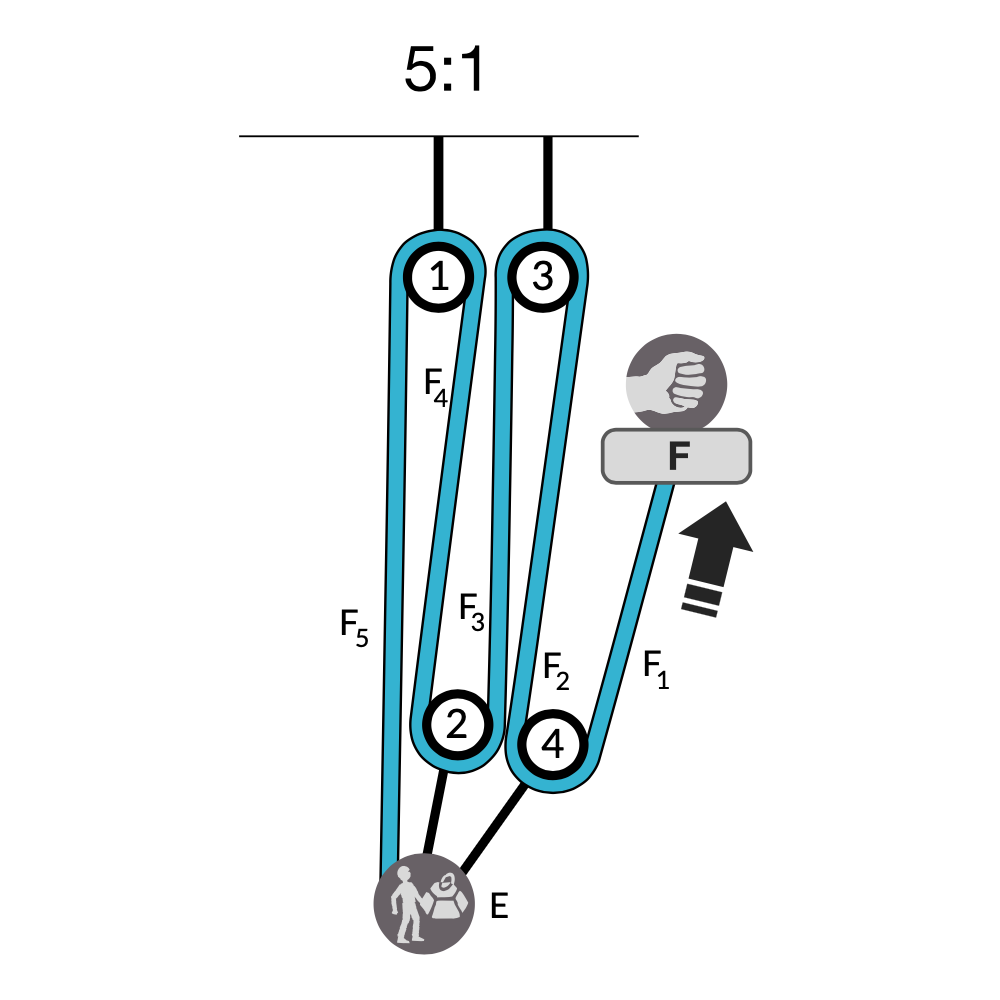
\includegraphics[width=10.0cm]{Figures/5_1/3_haul_syste_5_1_changed.png}
    \caption[Schéma kladkostroje 5:1]{Schéma kladkostroje 5:1 (schéma převzato ze zdroje \cite{Petzl_2022})}
    \label{Obr:pulley_system_5_1}
\end{figure} 
%% -------------------------------------------------- %%

\noindent Pro \textbf{systém 5:1} uvažuji následující vzorce:
%% -------------------------------------------------- %%
%% -------------------- Equation --------------------- %%
%% -------------------------------------------------- %%
\begin{equation}
    \label{eqn:9_calculation_5_1}
    F = \frac{m}{F_{celk}}
\end{equation}

\noindent Získáme následující rovnici, se kterou počítám ve webové aplikaci.
%% -------------------------------------------------- %%
%% -------------------- Equation --------------------- %%
%% -------------------------------------------------- %%
\begin{equation}
    \label{eqn:10_calculation_5_1}
    F = \frac{m}{1 + \frac{f_4}{100} \cdot (1 + \frac{f_3}{100} \cdot (1 + \frac{f_2}{100} \cdot (1 + \frac{f_1}{100})))}
\end{equation}
\subsection{Kladkostroj 7:1}
Uvažuji rozložení sil (viz~\autoref{Obr:pulley_system_7_1}). Od pramene, kterým se vytahuje zachraňovaný se jednotlivé části lana mezi kladkami rozdělí na ${F_1}$ - ${F_5}$. Kladky označuji ${f_1}$ - ${f_3}$ a začínají s číslováním od zachraňovaného.
%% -------------------------------------------------- %%
%% -------------------- Picture --------------------- %%
%% -------------------------------------------------- %%
\begin{figure}[!hbt]
    \centering
    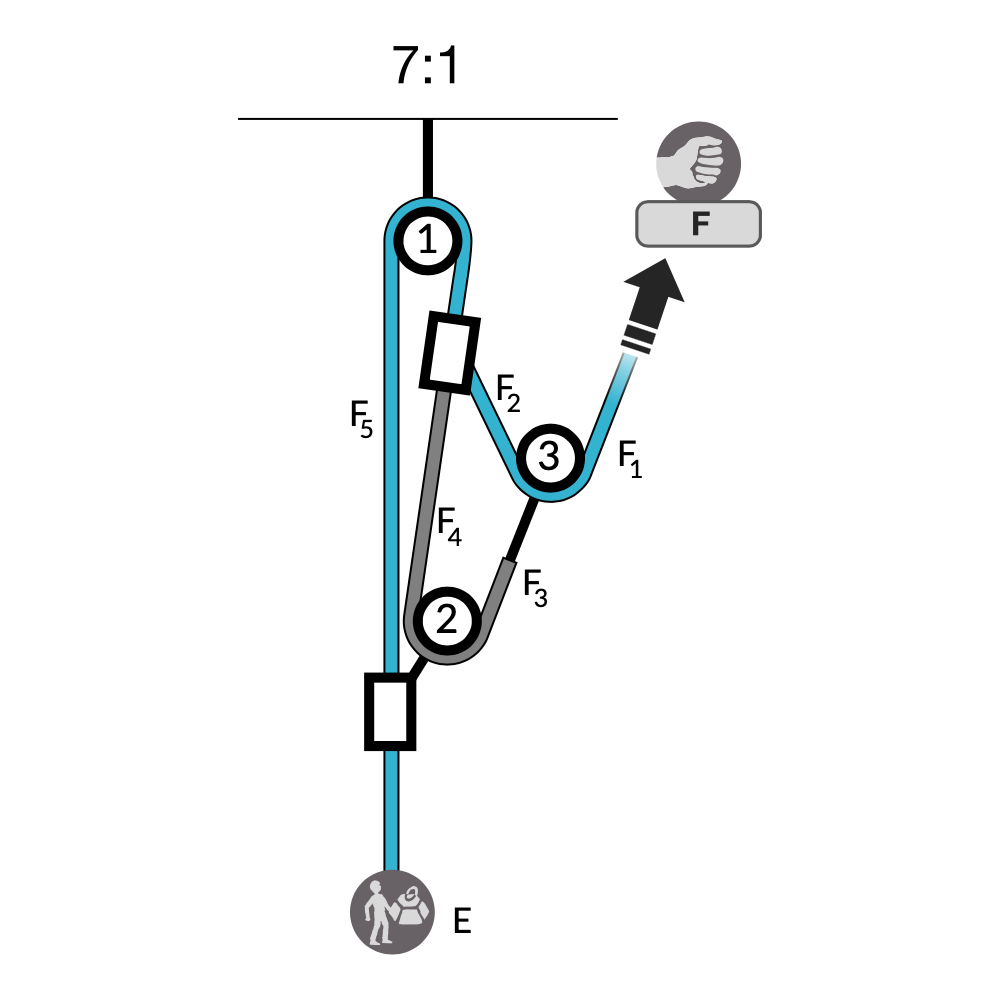
\includegraphics[width=10.0cm]{Figures/7_1/3_haul_syste_7_1_changed.png}
    \caption[Schéma kladkostroje 7:1]{Schéma kladkostroje 7:1 (schéma převzato ze zdroje \cite{Petzl_2022})}
    \label{Obr:pulley_system_7_1}
\end{figure} 
%% -------------------------------------------------- %%
\newpage
\noindent Pro \textbf{systém 7:1} uvažuji následující vzorce:
%% -------------------------------------------------- %%
%% -------------------- Equation --------------------- %%
%% -------------------------------------------------- %%
\begin{equation}
    \label{eqn:1_calculation_7_1}
    F_1 = 1
\end{equation}
%% -------------------------------------------------- %%
%% -------------------- Equation --------------------- %%
%% -------------------------------------------------- %%
\begin{equation}
    \label{eqn:2_calculation_7_1}
    F_2 = \frac{f_3}{100} \cdot F_1
\end{equation}
%% -------------------------------------------------- %%
%% -------------------- Equation --------------------- %%
%% -------------------------------------------------- %%
\begin{equation}
    \label{eqn:3_calculation_7_1}
    F_3 = F_1 + F_2
\end{equation}
%% -------------------------------------------------- %%
%% -------------------- Equation --------------------- %%
%% -------------------------------------------------- %%
\begin{equation}
    \label{eqn:4_calculation_7_1}
    F_4 = \frac{f_2}{100} \cdot F_3
\end{equation}
%% -------------------------------------------------- %%
%% -------------------- Equation --------------------- %%
%% -------------------------------------------------- %%
\begin{equation}
    \label{eqn:5_calculation_7_1}
    F_5 = \frac{f_1}{100} \cdot (F_2 + F_4)
\end{equation}
%% -------------------------------------------------- %%
%% -------------------- Equation --------------------- %%
%% -------------------------------------------------- %%
\begin{equation}
    \label{eqn:6_calculation_7_1}
    E = F_3 + F_4 + F_5
\end{equation}

\noindent Po dosazení do rovnice:
%% -------------------------------------------------- %%
%% -------------------- Equation --------------------- %%
%% -------------------------------------------------- %%
\begin{equation}
    \label{eqn:7_calculation_7_1}
    F_{celk} = (F_1 + F_2) + (\frac{f_2}{100} \cdot F_3) + (\frac{f_1}{100} \cdot (F_2 + F_4))
\end{equation}

\noindent Získáme následující rovnici:
%% -------------------------------------------------- %%
%% -------------------- Equation --------------------- %%
%% -------------------------------------------------- %%
\begin{equation}
    \label{eqn:8_calculation_7_1}
    F_{celk} = (1 + \frac{f_3}{100} \cdot 1) + (\frac{f_2}{100} \cdot (1 + (\frac{f_3}{100} \cdot 1))) + (\frac{f_1}{100} \cdot ((\frac{f_3}{100} \cdot 1) + (\frac{f_2}{100} \cdot (1 + (\frac{f_3}{100} \cdot 1)))))
\end{equation}

\noindent Dostávám následující rovnici, se kterou počítám ve webové aplikaci.
%% -------------------------------------------------- %%
%% -------------------- Equation --------------------- %%
%% -------------------------------------------------- %%
\begin{equation}
    \label{eqn:9_calculation_7_1}
    F = \frac{m}{F_{celk}}
\end{equation}

%% -------------------------------------------------- %%
%% -------------------- Equation --------------------- %%
%% -------------------------------------------------- %%
\begin{equation}
    \label{eqn:10_calculation_7_1}
    F = \frac{m}{(1 + \frac{f_3}{100} \cdot 1) + (\frac{f_2}{100} \cdot (1 + (\frac{f_3}{100} \cdot 1))) + (\frac{f_1}{100} \cdot ((\frac{f_3}{100} \cdot 1) + (\frac{f_2}{100} \cdot (1 + (\frac{f_3}{100} \cdot 1)))))}
\end{equation}

\begin{tabular}{l l c p{9.75cm}}
    kde: \hspace{0.25cm} & $F$ & -- & vytahovaná hmotnost zachraňovaného lezce [kg]\\
    \hspace{0.25cm} & $m$ & -- & hmotnost vytahovaného lezce [kg]\\
    \hspace{0.25cm} & $F_1$ - $F_5$ & -- & mezivýpočet účinnosti systému [\%]\\
    \hspace{0.25cm} & $f_1$ - $f_4$ & -- & účinnost kladkostroje [\%]\\
\end{tabular}
\\
\section{Výpočet vytažené délky lana k zachránění lezce o požadovanou vzdálenost}
Při výpočtu vycházím z již vypočtených účinností systému $F_{celk}$.
%% -------------------------------------------------- %%
%% -------------------- Equation --------------------- %%
%% -------------------------------------------------- %%
\begin{equation}
    \label{eqn:calculation_distance}
    l = l_{poz} \cdot F_{celk}
\end{equation}

\begin{tabular}{l l c p{9.75cm}}
    kde: \hspace{0.25cm} & $l$ & -- & skutečná vytažená délka lana k zachraně lezce o požadovanou vzdálenost [m]\\
    \hspace{0.25cm} & $l_{poz}$ & -- & požadovaná vzdálenost k vytažení zachraňovaného lezce [m]\\
    \hspace{0.25cm} & $F_{celk}$ & -- & celkový výpočet účinnosti systému [\%]\\
\end{tabular}